\documentclass[12pt]{article}
\usepackage{geometry}
\geometry{
	left=20mm,
	top=20mm,
}
\usepackage{cite}
\usepackage[utf8]{inputenc}
\usepackage[shortlabels]{enumitem}
\usepackage{array}
\newcolumntype{C}[1]{>{\centering\let\newline\\\arraybackslash\hspace{0pt}}m{#1}}
\usepackage[spanish,es-nodecimaldot]{babel}
 \usepackage{url}
\usepackage[spanish, fixlanguage]{babelbib}
\bibliographystyle{IEEEtran}
\usepackage{graphicx}
\graphicspath{ {./images/} }
\usepackage{amssymb}
\usepackage{amsmath}
\usepackage{subcaption}
\usepackage[linesnumbered]{algorithm2e}
\newcommand\mycommfont[1]{\footnotesize\ttfamily\textcolor{blue}{#1}}
\SetCommentSty{mycommfont}
\usepackage{tikz}
\usetikzlibrary{positioning, fit}
\usetikzlibrary{babel}
\usepackage{titlesec}
\titlespacing*{\section}
{0pt}{5.5ex plus 1ex minus .2ex}{.3ex plus .1ex}
\titlespacing*{\subsection}
{0pt}{5.5ex plus 1ex minus .2ex}{2.3ex plus .1ex}
\title{Propuesta de Proyecto Final:\\
	Estimación de nota musical}

\author{
	Saul Ivan Rivas Vega \\
	\\
	Aprendizaje Automatizado\\
}

\date{\today}

\begin{document}
	\maketitle
	\pagebreak
	\section{Descripción y delimitación del problema}
	  \paragraph{} Basado en atributos en el dominio de la frecuencia como son los coeficientes por ventana de muestreo de la transformada \textbf{constante-Q} estimar la nota musical de guitarra presente en un archivo de audio de una pieza musical monofónica con notas simples.
	\section{Objetivos}
	\begin{itemize}
	\item Extraer los atributos frecuenciales por ventana del conjunto de datos.
	\item Entrenar un modelo predictivo para estimar la nota musical presente en una ventana dados sus atributos frecuenciales.
	\item Realizar un transcript de alguna melodía pre-grabada.
	\end{itemize}
	\section{Justificación}
	\paragraph{} Se han realizado múltiples estudios en la estimación de frecuencia fundamental o de tono \cite{das_real-time_2017,kim_crepe_2018,mauch_pyin_2014,de_cheveigne_yin_2002}. En aplicaciones el ser en tiempo real como en \cite{das_real-time_2017} sería de gran utilidad, sin embargo los métodos con mayor precisión son los que analizan archivos pre-grabados como es el caso de \cite{kim_crepe_2018,mauch_pyin_2014}, ambos superando al método estándar YIN \cite{de_cheveigne_yin_2002} que se encuentra en múltiples bibliotecas de extracción de información musical como ESSENTIA \cite{bogdanov_essentia_2013}.\\
	El presente trabajo tiene como justificación el poder utilizar las propiedades fundamentales para la estimación del tono como en \cite{de_cheveigne_yin_2002,brown_calculation_1991,brown_efficient_1992} y a su vez beneficiarse de los métodos de aprendizaje automatizado para ofrecer una opción para la estimación de notas musicales balanceando la eficiencia en la cantidad de atributos requeridos y la precisión de la estimación, lo cual podría dejar una base para un sistema posterior para análisis en tiempo real.
	\section{Base de datos a utilizar o estrategia para recopilarla}
	\paragraph{} La base de datos es NSynth del grupo de investigación musical \textbf{Magenta} en Google \cite{engel_neural_2017}, el dataset contiene 305,979 notas musicales, cada una con un distinto tono, timbre, y envoltura, obtenidos de 1,006 instrumentos grabando clips de monofónicos con una taza de muestreo de 16kHz de 4 segundos con anotaciones de nota musical en el rango del formato MIDI (21-108) con 5 velocidades (25, 50, 75, 100, 127). La nota se mantuvo por 3 segundos dejando el último segundo para el decaimiento.
	\pagebreak
	\section{Análisis exploratorio de los datos}
	Para obtener un subconjunto del dataset se seleccionaron los clips de audio que cumplieran:
	\begin{itemize}
		\item  Su nota estuviera entre Do1 (C1) y Do4 (C4), de esta forma la resolución frecuencial podrá extraer valores de los armónicos, por ejemplo Do8 (C8) esta al borde y todos sus armónicos posteriores se pierden en nuestra resolución.
		\item Fueran de guitarra acústica, esto permitiría pruebas en entornos reales mas fácilmente.
		\item Su velocidad fuera de 127, es decir que la nota se tocó con la mayor potencia posible.
	\end{itemize}
	Lo cual da un total de 814 clips de audio, provenientes de 22 instrumentos tocando cada uno las 37 notas del rango a velocidad 127.\\
	
	De los clips de audio seleccionados se obtuvieron los valores de la transformada \textbf{Constante-Q} utilizando la biblioteca Librosa\cite{mcfee_librosa_2015} para python.
	
	Como el ejemplo de la figura \ref{fig1}, en el cual se muestran los componentes frecuenciales de un clip de audio correspondiente a la nota Do4 (C4) de una guitarra acústica.\\
	\begin{figure}[h!]
		\centering
		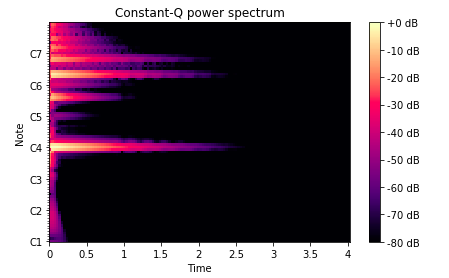
\includegraphics[width=.8\linewidth]{qtransform}
		\caption{Transformada \textbf{Constante-Q}.}
		\label{fig1}
	\end{figure}
\\
	Se organizaron en un Data Frame los atributos frecuenciales de las primeras 4 ventanas de muestreo (aproximadamente 1 segundo), añadiendo al final la clase a la que pertenece (la nota MIDI).\\
	El Data Frame terminó con 3256 registros 4 por cada clip, con sus respectivas componentes frecuenciales de la transformada las cuales van de la nota 24 (Do1, C1) hasta la nota 107 (Do8, C8) y finalmente mostrando en la última columna su clase, que en este caso es la nota en el rango MIDI de 24 a 60 (Do1-Do4, C1-C4).
	
	\begin{figure}[h!]\label{fig2}
	\centering
	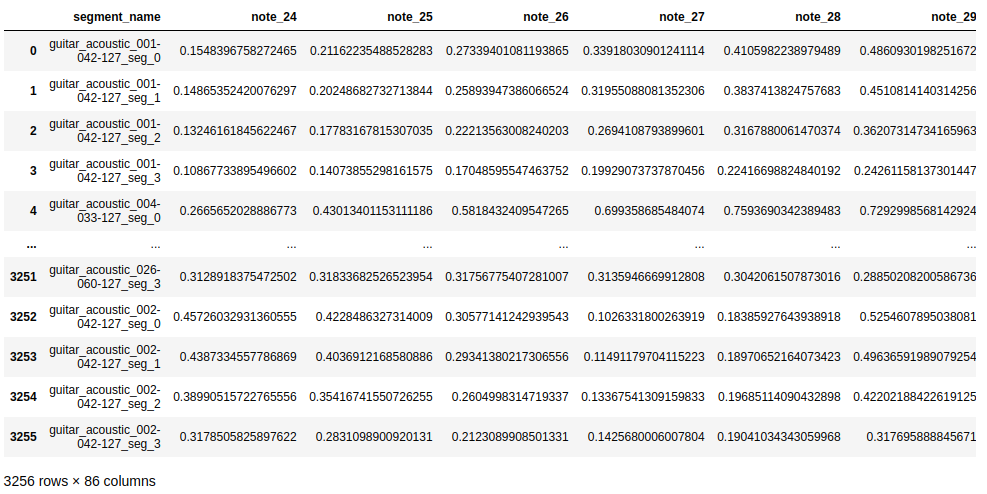
\includegraphics[width=.82\linewidth]{qtransfomtable_01}
	\caption{DataFrame con los datos.}
\end{figure}
	\begin{figure}[h!]\label{fig3}
	\centering
	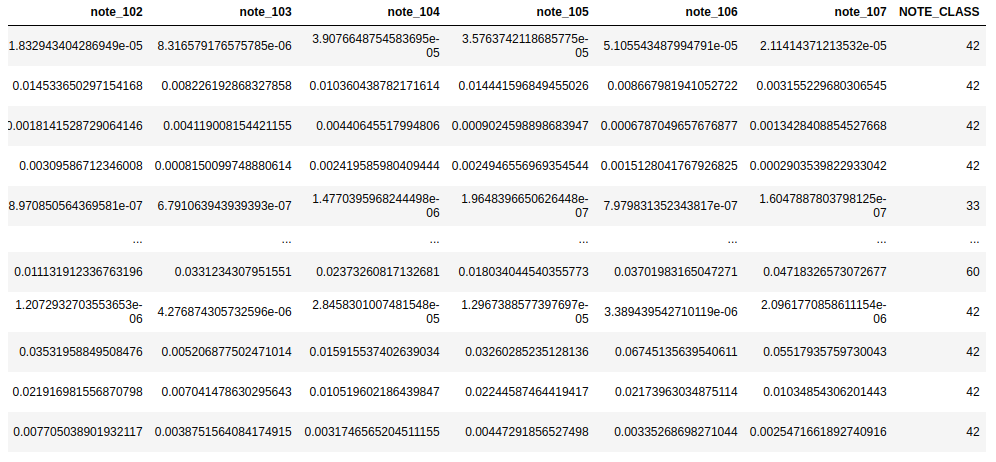
\includegraphics[width=.82\linewidth]{qtransformtable_02}
	\caption{DataFrame con los datos, mostrando la clase en la última columna.}
\end{figure}
\clearpage
	\bibliography{main}
\end{document}  